\documentclass[aspectratio=169,usepdftitle=true]{beamer}

\usepackage[T1]{fontenc}
\usepackage[utf8]{inputenc}
\usepackage{microtype}
\DisableLigatures{encoding = *, family = * }
\usepackage[english]{babel}
\usepackage{lipsum}
\usetheme[progressbar=foot]{metropolis}
%\usepackage{lmodern}

%\usepackage[default,type1,semibold]{sourcesanspro}
%\usepackage[sfdefault,semibold]{cabin}
%\usepackage[sfdefault]{AlegreyaSans}
\usepackage[sfdefault,lf,t]{carlito} % Looks nice! The only potential contender to lmodern!

\usepackage{mathpazo}
\usepackage{mathtools,calc} % For making colon symbol with the width of an equivalence rel.
%\usepackage[backend=bibtex8,style=alphabetic]{biblatex}
%\addbibresource{cutt-primer.bib}

%\usepackage[tabular,lining]{montserrat}
%\usepackage{InriaSans}
%\usepackage{domitian}
%\def\sbfamily{\fontfamily{Montserrat-TLF}\fontseries{sb}\selectfont}

%\usepackage{FiraSans}
%\firaextralight
% Titlepage Colors
%\setbeamercolor{title}{parent=normal text}
%\setbeamercolor{subtitle}{parent=normal text}
%\setbeamercolor{institute}{parent=normal text,fg=gray}
%\setbeamercolor{license}{parent=normal text,fg=gray}
%\setbeamercolor{tag}{parent=normal text,fg=gray}
%\setbeamercolor{date}{parent=normal text,fg=gray}

% Content
%\setbeamercolor{frametitle}{}
%\setbeamerfont{frametitle}{size=\Large,series=\mdseries}

% Titlepage Fonts
%\setbeamerfont{title}{size=\fontsize{24}{24},series=\sbfamily}
%\setbeamerfont{subtitle}{size=\fontsize{10}{12},series=\mdseries}
%\setbeamerfont{tag}{size=\fontsize{8}{10},series=\mdseries}
%\setbeamerfont{institute}{size=\fontsize{8}{10},series=\mdseries}
%\setbeamerfont{date}{size=\fontsize{8}{10},series=\mdseries}
%\setbeamerfont{section title}{size=\0fontsize{19}{19}}
%f\setbeamerfont{license}{size=\fontsize{6}{8},series=\mdseries}

% Navigation Symbols (Broken in this theme?)
%\setbeamertemplate{navigation symbols}{
%\insertframenavigationsymbol%
%}

\usepackage{xcolor}
\usepackage{mdframed}
\newmdenv[%
	innerleftmargin=4pt,
	innertopmargin=4pt,
	innerrightmargin=4pt,
	innerbottommargin=4pt,
	backgroundcolor=yellow!10,
]{boxybox}%
\usepackage{tabularx}

% ----------------------------------------------------

\title{Cubical Type Theory}
\subtitle{An Informal Introduction}
%\institute{Should I put "University of Cambridge" here?}
\date{November 30, 2022}
\author{Aaron Yeoh Cruz}

\newlength{\mywidth}
\newlength{\myheight}
\setlength{\mywidth}{85mm}
\setlength{\myheight}{112mm}

% ----------------------------------------------------

\newcommand{\defcolon}{\mathrel{\mathmakebox[\widthof{$\equiv$}]{:}}}
\newcommand{\entails}{\vdash}
\newcommand{\pathcom}{\mathbin{\vcenter{\hbox{\text{\tiny{$\bullet$}}}}}}

\newcommand{\interrule}{\centerline{\rule{\textwidth}{0.4pt}}}
\newcommand{\cleanalign}[2]{
	{#1
	\(\displaystyle
		#2
	\)
	\par}
}

% ----------------------------------------------------

% TikZ settings:

\usetikzlibrary{calc,positioning}
% Color of shapes used:
\definecolor{color_fill_default}{HTML}{d1d2e8}
\definecolor{color_shaded_default}{HTML}{888bc3}

\definecolor{color_heliotrope}{HTML}{dc85ff}
\definecolor{baby_powder}{HTML}{fdfffc}
\definecolor{color_flame}{HTML}{ee5622}
\definecolor{color_electric_purple}{HTML}{ba0aff}

\definecolor{color_cerulean_crayola}{HTML}{00a7e1}
\definecolor{color_blue}{HTML}{0410f1}
\definecolor{color_black_1b_2022}{HTML}{1b2022}
\definecolor{color_black_fogra}{HTML}{080708}
\definecolor{color_mbgreen}{HTML}{75dbcd}
\definecolor{color_msgreen}{HTML}{94da97}
\newcommand\drawsquare[1]{+(-#1,-#1) rectangle +(#1,#1)}

% ----------------------------------------------------

\setbeamercolor{background canvas}{bg=baby_powder}
\setbeamercolor{frametitle}{bg=color_black_1b_2022,fg=baby_powder}
\setbeamercolor{normal text}{fg=color_black_fogra}
\setbeamercolor{alerted text}{fg=color_flame}


\usepackage{array, booktabs, longtable}
\usepackage{graphicx}
\usepackage{colortbl}
\newcommand{\timelinebullet}{\color{color_black_fogra}\makebox[0pt]{\textbullet}\hskip-0.45pt\color{color_black_fogra}\vrule width 1pt\hspace{\labelsep}}

\usepackage{mathpartir}

\usepackage{soul}
\makeatletter
\let\HL\hl
\renewcommand\hl{%
  \let\set@color\beamerorig@set@color
  \let\reset@color\beamerorig@reset@color
  \HL}
\makeatother
\newcommand{\hlmathy}[2]{\text{\sethlcolor{#1}\hl{$#2$}}}

\usepackage[backend=bibtex8,style=alphabetic]{biblatex}
\addbibresource{cutt-primer.bib}

\begin{document}
% Start slide numbering at zero.
\addtocounter{framenumber}{-1}
\begin{frame}[plain]
	\titlepage
\end{frame}

%\section{Section}
%\subsection{Subsection}
\begin{frame}{Chronology}
	\begin{table}
		\renewcommand\arraystretch{1.4}
		\begin{tabular}{@{\,}r <{\hskip 2pt} !{\timelinebullet} >{\raggedright\arraybackslash}p{0.6\textwidth}}
		2013 & [BCH] “A Model of Type Theory in Cubical Sets”\\
		2015 & [CCHM] De Morgan Cubical Type Theory\\
		2018 & [CHM] Higher Inductive Types in CuTT\\
		2019 & [VMA] Cubical Agda\\
		\end{tabular}
	\end{table}
\end{frame}

\begin{frame}<1-5>[t]{Sets as Types}
	\centering
	\bgroup
	{
		\def\arraystretch{1.5}
		\begin{tabularx}{\textwidth}{@{}>{\centering\arraybackslash}X|>{\centering\arraybackslash}X@{}}
			\textbf{Types} & \textbf{Sets}\\\hline
			$x : A$ & $x \in A$
			\only<2->{\\\hline
			\textcolor<3-4>{gray}{$\mathbf{0}$} & \textcolor<3-4>{gray}{$\emptyset$} \\
			\textcolor<3-4>{gray}{$\mathbf{1}$} & \textcolor<3-4>{gray}{$\{0\}$} \\
			\textcolor<4>{gray}{\alt<3>{$\mathsf{inl}\, x : A + B$}{$A + B$}} & \textcolor<4>{gray}{\alt<3>{$(0, x) \in A \uplus B$}{$A \uplus B$}} \\
			\textcolor<3>{gray}{\alt<4>{$(x, y) : A \times B$}{$A \times B$}} & \textcolor<3>{gray}{\alt<4>{$(x, y) \in A \times B$}{$A \times B$}} \\
			\textcolor<3-4>{gray}{$A \to B$} & \textcolor<3-4>{gray}{$B^A$} \\
			}
		\end{tabularx}
	}
	\egroup
\end{frame}

\begin{frame}<1-6>[t]{Propositions as Types}
	\centering
	\bgroup
	{
		\def\arraystretch{1.5}
		\begin{tabularx}{\textwidth}{@{}>{\centering\arraybackslash}X|>{\centering\arraybackslash}X@{}}
			\textbf{Types} & \textbf{Propositions}\\\hline
			$x : A$ & $A \mathrel{\mathsf{true}}$
			\only<2->{\\\hline
			\textcolor<3-4>{gray}{$\mathbf{0}$} & \textcolor<3-4>{gray}{$\bot$} \\
			\textcolor<3-4>{gray}{$\mathbf{1}$} & \textcolor<3-4>{gray}{$\top$} \\
			\textcolor<3-4>{gray}{$A + B$} & \textcolor<3-4>{gray}{$A \lor B$} \\
			\textcolor<4>{gray}{\alt<3>{$(x, y) : A \times B$}{$A \times B$}} & \textcolor<4>{gray}{\alt<3>{$A \land B \mathrel{\mathsf{true}}$}{$A \land B$}} \\
			\textcolor<3>{gray}{\alt<4>{$\lambda x.\,y : A \to B$}{$A \to B$}} & \textcolor<3>{gray}{\alt<4>{$A \implies B \mathrel{\mathsf{true}}$}{$A \implies B$}} \\
			}
		\end{tabularx}
	}
	\egroup

	\only<6>{This translation is known as the \textbf{Curry-Howard correspondence}.}
\end{frame}

\begin{frame}{Propositions as Types | Agda}
	\centering
	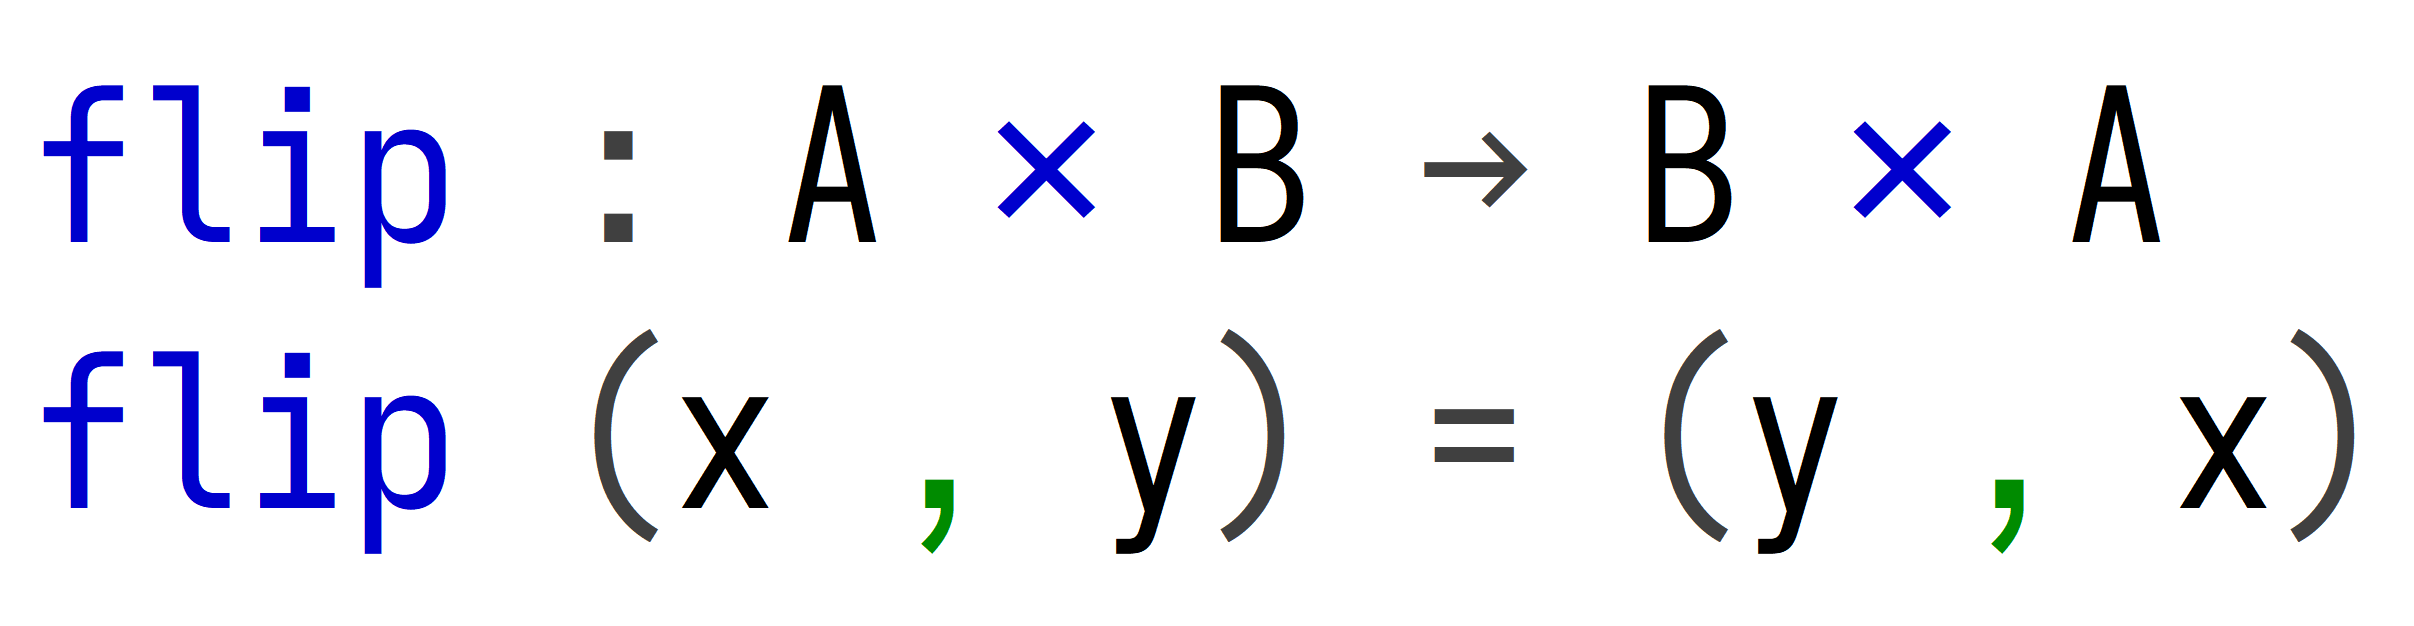
\includegraphics[height=32pt]{../res/flip-simple.png}
\end{frame}

\begin{frame}{Universes and Quantifiers}
	We're still missing some crucial type formers:
	\begin{itemize}
		\uncover<2->{\item We don't have a way to talk about types \textbf{internally}.}
		\uncover<3->{\item We don't have existential/universal \textbf{quantifiers}.}
	\end{itemize}
\end{frame}

\begin{frame}<1-3>{Universes}
	\centering
	\alt<1-2>{
		We'll add a \textbf{universe}\dots
		\begin{equation*}
			\mathcal{U}
		\end{equation*}
	}{
		We'll add a \emph{hierarchy} of \textbf{universes}\dots
		\begin{equation*}
			\mathcal{U}_0 : \mathcal{U}_1 : \mathcal{U}_2 : \cdots
		\end{equation*}
	}
	\uncover<2->{\dots closed under our type formers.}
\end{frame}

\begin{frame}<1-6>[t]{Quantifiers}
	\centering
	A \textbf{type family} $P : A \to \mathcal{U}$ represents a \textbf{predicate}.
	\vspace*{\baselineskip}

	\uncover<2->{
	\alt<2-5>{
	\bgroup
	\def\arraystretch{1.5}
	\begin{tabularx}{\textwidth}{@{}>{\centering\arraybackslash}X|>{\centering\arraybackslash}X@{}}
		\textbf{Types} & \textbf{Propositions}\\\hline
		\only<3->{$\displaystyle(x, y) : \sum_{x : A}\,P\, x$} & $\displaystyle\vphantom{\sum_{x : A}}\exists x.(x \in A) \land P(x)$
		\only<4->{\\
			\only<5->{$\displaystyle\lambda x.\, y : \prod_{x : A}\,P\, x$} & $\displaystyle\vphantom{\prod_{x : A}}\forall x.(x \in A) \implies P(x)$
		\\}
	\end{tabularx}
	\egroup
	}{
	\bgroup
	\def\arraystretch{1.5}
	\begin{tabularx}{\textwidth}{@{}>{\centering\arraybackslash}X|>{\centering\arraybackslash}X|>{\centering\arraybackslash}X@{}}
		\textbf{Sets} & \textbf{Types} & \textbf{Propositions}\\\hline
		$\displaystyle\biguplus_{x \in A}\, P(x)$ & $\displaystyle\sum_{x : A}\,P\, x$ & $\displaystyle\exists x.(x \in A) \land P(x)$\\
		$\displaystyle\prod_{x \in A}\, P(x)$ & $\displaystyle\prod_{x : A}\,P\, x$ & $\displaystyle\forall x.(x \in A) \implies P(x)$\\
	\end{tabularx}
	\egroup
	}
	}
\end{frame}


\begin{frame}{Dependent Types | Agda}
	\centering
	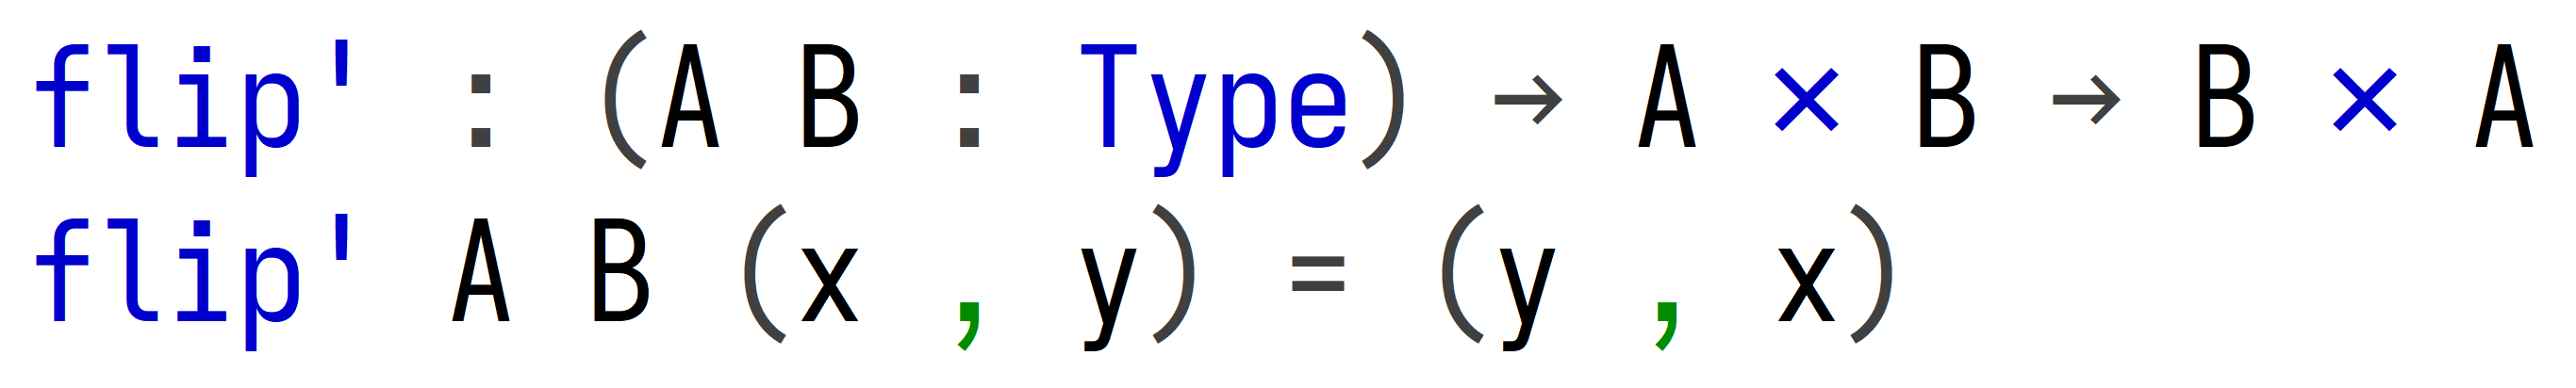
\includegraphics[height=32pt]{../res/flip-dependent.png}
\end{frame}

\begin{frame}<1-2>[label=wbequality]{What About Equality?}
	\centering
	\cleanalign{\centering}{
		\begin{gathered}
			\overbrace{\mathbf{0}\qquad\mathbf{1}\qquad\mathbf{2}\qquad\mathbb{N}\qquad{+}\qquad{\Sigma}\qquad{\times}}^\text{inductive types}\qquad{\Pi}\qquad\mathcal{U}
		\end{gathered}
	}
	
	\vspace*{\baselineskip}
	\interrule

	\uncover<2->{We'd like a type $x = y$ whose terms \textbf{witness} the fact that $x$ equals $y$.}

	\uncover<3->{Cubical type theories take inspiration from \textbf{topology}.}
\end{frame}

\begin{frame}{The Martin-L"of Identity Type}
	\centering
	We could encode equality as an \textbf{indexed inductive} \emph{identity} type.

	\bigskip
	\uncover<2->{
	
\includegraphics[height=32pt]{../res/mltt-id.png}
	}

	\uncover<3->{
	This is elegant in some ways (\emph{judgemental} path induction)\dots
	}

	\uncover<4->{
	\dots but inadequate in others (lacks \textbf{function extensionality}).
	}
\end{frame}

\againframe<3->{wbequality}

\begin{frame}{Paths, Topologically}
	\medskip
	
	\begin{columns}[b,onlytextwidth]
		\begin{column}{0.6666\textwidth}
			\centering
			\uncover<2->{
				A \textbf{path} $p$ in a topological space $X$ is a continuous map
				\begin{equation*}
				p : \mathbb{I} \to X
				\end{equation*}
				where $\mathbb{I}$ is the \textbf{unit interval} $[0, 1]$.
			}
		\end{column}
		\begin{column}{0.3333\textwidth}
			\centering
			\uncover<2->{
				\begin{tikzpicture}[scale=1,black,y=-1cm,every node/.style={scale=0.6}]
					% Points
					\coordinate (Z) at (0.5000, -0.4);
					\coordinate (U) at (1.5000, -0.4);
					\coordinate (A) at (0.5000, 0.5000);
					\coordinate (B) at (1.5000, 1.2000);

					% Space
					\draw[black,line width=1pt,fill=color_fill_default] plot [smooth cycle] coordinates {
					(1.8756, 0.6404)
					(1.1386, 0.0481)
					(0.2441, 0.2829)
					(0.0758, 1.2369)
					(0.8278, 1.9409)
					(1.7991, 1.6066)
					};
					\draw (0, 1) node[left=1pt] {$X$};
					
					% Interval
					\uncover<3->{
					\draw (Z) -- (U);

					\draw (Z) node[left=1pt] {$\mathbb{I}$};
					\draw ($(Z)+(0,0.05)$) -- ($(Z)+(0,-0.05)$) node[above] {$0$};
					\draw ($(U)+(0,0.05)$) -- ($(U)+(0,-0.05)$) node[above] {$1$};
					}

					% Path
					\only<2->{
						\draw[black, line width=1pt]
							(A)
								.. controls (1.046, 0.616) and (0.984, 1.142) ..
							(B);
						\draw (1, 1) node[below left] {$p$};
					}

					% Endpoints
					\only<4->{
						\draw[dashed] (Z) -- (A);
						\draw[dashed] (U) -- (B);
						\fill[black] (A) circle(1.4pt) node[below=1pt] {$p_0$};
						\fill[black] (B) circle(1.4pt) node[below=1pt] {$p_1$};
					}
				\end{tikzpicture}
			}
		\end{column}
	\end{columns}

	\interrule

	\uncover<5->{
		\centering
		What if we treat a type as a kind of space,

		where two points are \textit{equal} iff they are connected by a path?
		\par
	}
\end{frame}
\begin{frame}{The (De Morgan) Interval}
	\centering
	\uncover<2->{
	We define an \alert{exotype} $\mathbb{I}$, such that:
	
	\cleanalign{\centering}{
		\begin{gathered}
			0, 1 : \mathbb{I}
		\end{gathered}
	}
	}

	\uncover<3->{and equip it with \textbf{connections} \uncover<4->{and a \textbf{reversal}.}}%

	\interrule

	\vspace{\baselineskip}

	\begin{columns}[onlytextwidth]
		\begin{column}{0.5\textwidth}
			\uncover<3->{
			\cleanalign{\centering}{
				\begin{gathered}
					r \lor s : \mathbb{I}\\
					r \land s : \mathbb{I}
				\end{gathered}
			}
			\centering
			
			\vspace{\baselineskip}

			for any $r, s : \mathbb{I}$
			}
		\end{column}
		\begin{column}{0.5\textwidth}
			\uncover<4->{
			\cleanalign{\centering}{
				\begin{gathered}
					\neg t : \mathbb{I}
				\end{gathered}
			}
			\centering
			
			\vspace{\baselineskip}

			for any $t : \mathbb{I}$
			}
		\end{column}
	\end{columns}
\end{frame}

\begin{frame}{The Interval, Morally}
	A \textbf{dimension term} $r : \mathbb{I}$ can be thought of as an point $r \in [0, 1]$.

	\begin{itemize}
		\uncover<2->{
			\item \textbf{Max connection.} $r \lor s $ represents $\mathsf{max}(r, s)$
			\item \textbf{Min connection.} $r \land s$ represents $\mathsf{min}(r, s)$
		}
		\uncover<3->{
			\item \textbf{Reversal.} $\neg r \approx 1 - r$
		}
	\end{itemize}
\end{frame}

\begin{frame}{Points, Lines, Squares, Cubes}
	\centering
	In any context $\Gamma$,
	we have $n$ \textbf{dimension variables} $i : \mathbb{I} \in \Gamma$.
	
	\uncover<2->{
	A term $\Gamma \entails x : A$ looks like:
	}
	\vspace*{\baselineskip}

	\begin{columns}[t,onlytextwidth]
		\uncover<2->{
		\begin{column}{0.333\textwidth}
			\centering
			\begin{tikzpicture}[scale=1,black,x=1pt,y=1pt,every node/.style={scale=0.6}]
				\useasboundingbox (-32, -4) rectangle (80, 80);
				\fill[color_shaded_default]
					(24, 48) circle(2pt)
					;
			\end{tikzpicture}
		\end{column}
		}
		\uncover<3->{
		\begin{column}{0.333\textwidth}
			\centering
			\begin{tikzpicture}[scale=1,black,x=1pt,y=1pt,every node/.style={scale=0.6}]
				\useasboundingbox (-32, -4) rectangle (80, 80);
				% Points
				\coordinate (TL) at (0, 48);
				\coordinate (TR) at (48, 48);
		
				\coordinate (ZI) at ($(TL) + (0, 16)$);
				\coordinate (UI) at ($(TR) + (0, 16)$);
		
				% Square background
				\draw[line width=0,fill=color_fill_default]
				(TL) --
				(TR);
				
				% Interval
				\draw (ZI) -- (UI);
				\draw ($(ZI)+(0,-2)$) -- ($(ZI)+(0,2)$) node[above] {$0$};
				\draw ($(UI)+(0,-2)$) -- ($(UI)+(0,2)$) node[above] {$1$};
				\draw ($(ZI)!0.5!(UI) + (0,2)$) node[above] {$i$}
				;
				
				% Grays
				\draw[line width=1.5pt, color_shaded_default]
					(TL) -- (TR)
					;
			\end{tikzpicture}
		\end{column}
		}
		\uncover<4->{
		\begin{column}{0.333\textwidth}
			\centering
			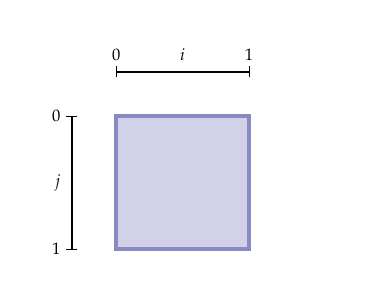
\begin{tikzpicture}[scale=1,black,x=1pt,y=1pt,every node/.style={scale=0.6}]
				\useasboundingbox (-32, -4) rectangle (80, 80);
				%\draw (-32, -4) rectangle (52, 80);
				% Points
				\coordinate (TL) at (0, 48);
				\coordinate (TR) at (48, 48);
				\coordinate (BR) at (48, 0);
				\coordinate (BL) at (0, 0);
		
				\coordinate (ZI) at ($(TL) + (0, 16)$);
				\coordinate (UI) at ($(TR) + (0, 16)$);
				\coordinate (ZJ) at ($(TL) + (-16, 0)$);
				\coordinate (UJ) at ($(BL) + (-16, 0)$);
				\coordinate (ZJR) at ($(TR) + (16, 0)$);
				\coordinate (UJR) at ($(BR) + (16, 0)$);
		
				% Square background
				\draw[line width=0,fill=color_fill_default]
				(TL) --
				(TR) --
				(BR) --
				(BL) --
				cycle;
				
				% Interval
				\draw (ZI) -- (UI);
				\draw ($(ZI)+(0,-2)$) -- ($(ZI)+(0,2)$) node[above] {$0$};
				\draw ($(UI)+(0,-2)$) -- ($(UI)+(0,2)$) node[above] {$1$};
				\draw ($(ZI)!0.5!(UI) + (0,2)$) node[above] {$i$}
				;
				\draw (ZJ) -- (UJ);
				\draw ($(ZJ)+(2, 0)$) -- ($(ZJ)+(-2, 0)$) node[left] {$0$};
				\draw ($(UJ)+(2,0)$) -- ($(UJ)+(-2, 0)$) node[left] {$1$};
				\draw ($(ZJ)!0.5!(UJ) + (-2, 0)$) node[left] {$j$};
				
				% Grays
				\draw[line width=1.5pt, color_shaded_default]
					(TL) -- (TR) -- (BR) -- (BL) -- cycle
					;
			\end{tikzpicture}
		\end{column}
		}
	\end{columns}
	\vspace*{\baselineskip}
	\uncover<5->{
	A \textbf{line} $i : I \entails x : A$ or $\lambda i.\, x :\mathbb{I} \to A$ \emph{witnesses} the equality of its endpoints.
	}
\end{frame}

\begin{frame}{Cofibrant Propositions}
	\begin{center}
	In any context $\Gamma$,
	we have a class $\mathbb{F}$ of
	
	\textbf{cofibrant propositions}, or \textbf{cofibrations}.
	
	\uncover<2->{We define $\mathbb{F}$ to be the \textbf{face lattice}.}
	\interrule
	\begin{columns}[onlytextwidth]
		\uncover<3->{
		\begin{column}{0.333\textwidth}
			\centering
			\begin{gather*}
				0_\mathbb{F}\\
				1_\mathbb{F}
			\end{gather*}
			\phantom{$\mathbb{I}$}
		\end{column}
		}
		\uncover<4->{
		\begin{column}{0.333\textwidth}
			\centering
			\begin{gather*}
				(i = 0)\\
				(i = 1)
			\end{gather*}
			for any $i : \mathbb{I}$ in $\Gamma$
		\end{column}
		}
		\uncover<5->{
		\begin{column}{0.333\textwidth}
			\centering
			\begin{gather*}
				\varphi \lor \psi\\
				\varphi \land \psi
			\end{gather*}
			for any $\varphi, \psi : \mathbb{F}$
		\end{column}
		}
	\end{columns}
	\end{center}
\end{frame}

\begin{frame}{Partial Elements}
	\centering
	If $\Gamma \entails \varphi : \mathbb{F}$ is a cofibration, \uncover<2->{then $\Gamma, \varphi$ is an \textbf{restricted context}.}
	
	\uncover<3->{We say that $\Gamma, \varphi \entails x : A$ is a \textbf{partial element} of $A$ (on the \alert{extent} of $\varphi$).}
	\vspace*{\baselineskip}
	\begin{columns}[onlytextwidth]
		\uncover<4->{
		\begin{column}{0.5\textwidth}
			\centering
			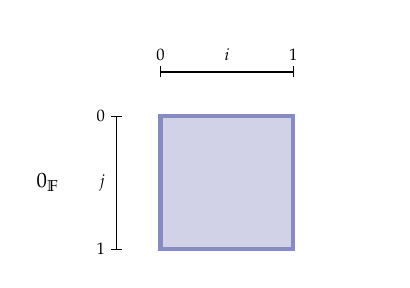
\begin{tikzpicture}[scale=1,black,x=1pt,y=1pt,every node/.style={scale=0.6}]
				\useasboundingbox (-48, -4) rectangle (80, 80);
				%\draw (-48, -4) rectangle (80, 80);
				% Points
				\coordinate (TL) at (0, 48);
				\coordinate (TR) at (48, 48);
				\coordinate (BR) at (48, 0);
				\coordinate (BL) at (0, 0);
		
				\coordinate (ZI) at ($(TL) + (0, 16)$);
				\coordinate (UI) at ($(TR) + (0, 16)$);
				\coordinate (ZJ) at ($(TL) + (-16, 0)$);
				\coordinate (UJ) at ($(BL) + (-16, 0)$);
				\coordinate (ZJR) at ($(TR) + (16, 0)$);
				\coordinate (UJR) at ($(BR) + (16, 0)$);
		
				% Square background
				\draw[line width=0,fill=color_fill_default]
				(TL) --
				(TR) --
				(BR) --
				(BL) --
				cycle;
				
				% Interval
				\draw (ZI) -- (UI);
				\draw ($(ZI)+(0,-2)$) -- ($(ZI)+(0,2)$) node[above] {$0$};
				\draw ($(UI)+(0,-2)$) -- ($(UI)+(0,2)$) node[above] {$1$};
				\draw ($(ZI)!0.5!(UI) + (0,2)$) node[above] {$i$}
				;
				\draw (ZJ) -- (UJ);
				\draw ($(ZJ)+(2, 0)$) -- ($(ZJ)+(-2, 0)$) node[left] {$0$};
				\draw ($(UJ)+(2,0)$) -- ($(UJ)+(-2, 0)$) node[left] {$1$};
				\draw ($(ZJ)!0.5!(UJ) + (-2, 0)$) node[left] {$j$}
				node[left=16pt,style={scale=1.25}] {$0_{\mathbb{F}}$};
				
				% Grays
				\draw[line width=1.5pt, color_shaded_default]
					(TL) -- (TR) -- (BR) -- (BL) -- cycle
					;
			\end{tikzpicture}
		\end{column}
		}
		\uncover<5->{
		\begin{column}{0.5\textwidth}
			\centering
			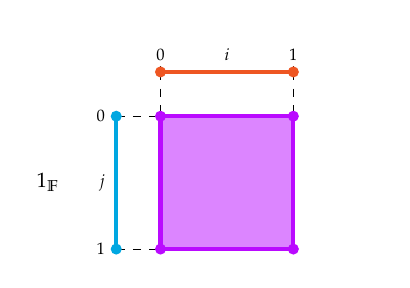
\begin{tikzpicture}[scale=1,black,x=1pt,y=1pt,every node/.style={scale=0.6}]
				\useasboundingbox (-48, -4) rectangle (80, 80);
				%\draw (-48, -4) rectangle (80, 80);
				% Points
				\coordinate (TL) at (0, 48);
				\coordinate (TR) at (48, 48);
				\coordinate (BR) at (48, 0);
				\coordinate (BL) at (0, 0);
		
				\coordinate (ZI) at ($(TL) + (0, 16)$);
				\coordinate (UI) at ($(TR) + (0, 16)$);
				\coordinate (ZJ) at ($(TL) + (-16, 0)$);
				\coordinate (UJ) at ($(BL) + (-16, 0)$);
				\coordinate (ZJR) at ($(TR) + (16, 0)$);
				\coordinate (UJR) at ($(BR) + (16, 0)$);
		
				% Square background
				\draw[line width=0,fill=color_heliotrope]
				(TL) --
				(TR) --
				(BR) --
				(BL) --
				cycle;
				
				% Interval
				\draw (ZI) -- (UI);
				\draw ($(ZI)+(0,-2)$) -- ($(ZI)+(0,2)$) node[above] {$0$};
				\draw ($(UI)+(0,-2)$) -- ($(UI)+(0,2)$) node[above] {$1$};
				\draw ($(ZI)!0.5!(UI) + (0,2)$) node[above] {$i$}
				;
				\draw (ZJ) -- (UJ);
				\draw ($(ZJ)+(2, 0)$) -- ($(ZJ)+(-2, 0)$) node[left] {$0$};
				\draw ($(UJ)+(2,0)$) -- ($(UJ)+(-2, 0)$) node[left] {$1$};
				\draw ($(ZJ)!0.5!(UJ) + (-2, 0)$) node[left] {$j$}
				node[left=16pt,style={scale=1.25}] {$1_{\mathbb{F}}$};
				
				% Dashed projections
				\draw[dashed]
					(ZI) -- (TL)
					(UI) -- (TR)
					(ZJ) -- (TL)
					(UJ) -- (BL)
					;
		
				% Highlights
				\draw[line width=1.5pt, color_electric_purple]
					(BL) -- (BR) -- (TR) -- (TL) -- cycle;
				\fill[color_electric_purple]
					(TL) circle(2pt)
					(TR) circle(2pt)
					(BL) circle(2pt)
					(BR) circle(2pt)
					;
				\draw[color_flame, line width=1.5pt]
					(ZI) -- (UI)
					;
				\fill[color_flame]
					(ZI) circle(2pt)
					(UI) circle(2pt)
					;
				\draw[color_cerulean_crayola, line width=1.5pt]
					(ZJ) -- (UJ)
					;
				\fill[color_cerulean_crayola]
					(ZJ) circle(2pt)
					(UJ) circle(2pt)
					;
			\end{tikzpicture}
		\end{column}
		}
	\end{columns}
\end{frame}

\begin{frame}{Example | Cofibrations}
	\centering
	\begin{columns}
		% (i = 0)
		\uncover<2->{
		\begin{column}{0.25\textwidth}
			\centering
			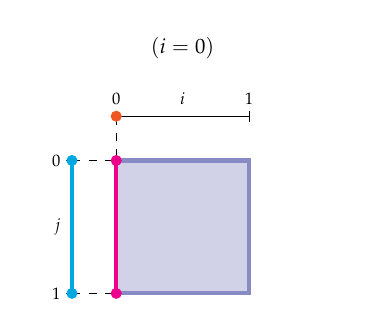
\begin{tikzpicture}[scale=1,black,x=1pt,y=1pt,every node/.style={scale=0.6}]
				\useasboundingbox (-32, -4) rectangle (80, 96);
				% Points
				\coordinate (TL) at (0, 48);
				\coordinate (TR) at (48, 48);
				\coordinate (BR) at (48, 0);
				\coordinate (BL) at (0, 0);
		
				\coordinate (ZI) at ($(TL) + (0, 16)$);
				\coordinate (UI) at ($(TR) + (0, 16)$);
				\coordinate (ZJ) at ($(TL) + (-16, 0)$);
				\coordinate (UJ) at ($(BL) + (-16, 0)$);
				\coordinate (ZJR) at ($(TR) + (16, 0)$);
				\coordinate (UJR) at ($(BR) + (16, 0)$);
		
				% Square background
				\draw[line width=0,fill=color_fill_default]
				(TL) --
				(TR) --
				(BR) --
				(BL) --
				cycle;
				
				% Interval
				\draw (ZI) -- (UI);
				\draw ($(ZI)+(0,-2)$) -- ($(ZI)+(0,2)$) node[above] {$0$};
				\draw ($(UI)+(0,-2)$) -- ($(UI)+(0,2)$) node[above] {$1$};
				\draw ($(ZI)!0.5!(UI) + (0,2)$) node[above] {$i$}
					node[above=16pt,style={scale=1.25}] {$(i = 0)$}
				;
				\draw (ZJ) -- (UJ);
				\draw ($(ZJ)+(2, 0)$) -- ($(ZJ)+(-2, 0)$) node[left] {$0$};
				\draw ($(UJ)+(2,0)$) -- ($(UJ)+(-2, 0)$) node[left] {$1$};
				\draw ($(ZJ)!0.5!(UJ) + (-2, 0)$) node[left] {$j$};
				
				% Dashed projections
				\draw[dashed]
					(ZJ) -- (TL)
					(UJ) -- (BL)
					(ZI) -- (TL)
					;
		
				% Grays
				\draw[line width=1.5pt, color_shaded_default]
					(TL) -- (TR) -- (BR) -- (BL) -- cycle
					;
		
				% Highlights
				\draw[line width=1.5pt, magenta]
					(TL) -- (BL);
				\fill[magenta]
					(TL) circle(2pt)
					(BL) circle(2pt)
					;
				\draw[color_flame, line width=1.5pt]
					(ZJ) -- (UJ)
					;
				\fill[color_flame]
					(ZI) circle(2pt)
					;
					
				\draw[color_cerulean_crayola, line width=1.5pt]
					(ZJ) -- (UJ)
					;
				\fill[color_cerulean_crayola]
					(ZJ) circle(2pt)
					(UJ) circle(2pt)
					;
			\end{tikzpicture}
		\end{column}
		}
		% (j = 1)
		\uncover<3->{
		\begin{column}{0.25\textwidth}
			\centering
			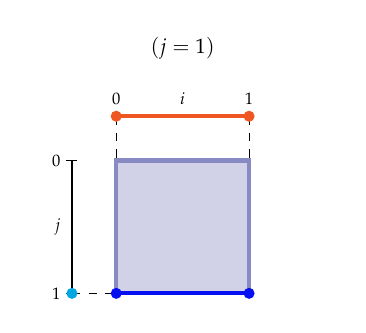
\begin{tikzpicture}[scale=1,black,x=1pt,y=1pt,every node/.style={scale=0.6}]
				\useasboundingbox (-32, -4) rectangle (80, 96);
				% Points
				\coordinate (TL) at (0, 48);
				\coordinate (TR) at (48, 48);
				\coordinate (BR) at (48, 0);
				\coordinate (BL) at (0, 0);
		
				\coordinate (ZI) at ($(TL) + (0, 16)$);
				\coordinate (UI) at ($(TR) + (0, 16)$);
				\coordinate (ZJ) at ($(TL) + (-16, 0)$);
				\coordinate (UJ) at ($(BL) + (-16, 0)$);
				\coordinate (ZJR) at ($(TR) + (16, 0)$);
				\coordinate (UJR) at ($(BR) + (16, 0)$);
		
				% Square background
				\draw[line width=0,fill=color_fill_default]
				(TL) --
				(TR) --
				(BR) --
				(BL) --
				cycle;
				
				% Interval
				\draw (ZI) -- (UI);
				\draw ($(ZI)+(0,-2)$) -- ($(ZI)+(0,2)$) node[above] {$0$};
				\draw ($(UI)+(0,-2)$) -- ($(UI)+(0,2)$) node[above] {$1$};
				\draw ($(ZI)!0.5!(UI) + (0,2)$) node[above] {$i$}
					node[above=16pt,style={scale=1.25}] {$(j = 1)$}
				;
				\draw (ZJ) -- (UJ);
				\draw ($(ZJ)+(2, 0)$) -- ($(ZJ)+(-2, 0)$) node[left] {$0$};
				\draw ($(UJ)+(2,0)$) -- ($(UJ)+(-2, 0)$) node[left] {$1$};
				\draw ($(ZJ)!0.5!(UJ) + (-2, 0)$) node[left] {$j$};
				
				% Dashed projections
				\draw[dashed]
					(ZI) -- (TL)
					(UI) -- (TR)
					(UJ) -- (BL)
					;
		
				% Grays
				\draw[line width=1.5pt, color_shaded_default]
					(TL) -- (TR) -- (BR) -- (BL) -- cycle
					;
		
				% Highlights
				\draw[color_blue, line width=1.5pt]
					(BL) -- (BR);
				\fill[color_blue]
					(BL) circle(2pt)
					(BR) circle(2pt)
					;
				\draw[color_flame, line width=1.5pt]
					(ZI) -- (UI)
					;
				\fill[color_flame]
					(ZI) circle(2pt)
					(UI) circle(2pt)
					;
				\fill[color_cerulean_crayola]
					(UJ) circle(2pt)
					;
			\end{tikzpicture}
		\end{column}
		}
		% (i = 0) OR (j = 1)
		\uncover<4->{
		\begin{column}{0.25\textwidth}
			\centering
			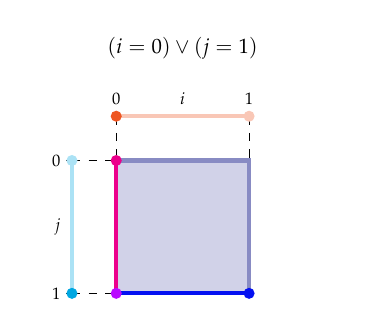
\begin{tikzpicture}[scale=1,black,x=1pt,y=1pt,every node/.style={scale=0.6}]
				\useasboundingbox (-32, -4) rectangle (80, 96);
				% Points
				\coordinate (TL) at (0, 48);
				\coordinate (TR) at (48, 48);
				\coordinate (BR) at (48, 0);
				\coordinate (BL) at (0, 0);
		
				\coordinate (ZI) at ($(TL) + (0, 16)$);
				\coordinate (UI) at ($(TR) + (0, 16)$);
				\coordinate (ZJ) at ($(TL) + (-16, 0)$);
				\coordinate (UJ) at ($(BL) + (-16, 0)$);
				\coordinate (ZJR) at ($(TR) + (16, 0)$);
				\coordinate (UJR) at ($(BR) + (16, 0)$);
		
				% Square background
				\draw[line width=0,fill=color_fill_default]
				(TL) --
				(TR) --
				(BR) --
				(BL) --
				cycle;
				
				% Interval
				\draw (ZI) -- (UI);
				\draw ($(ZI)+(0,-2)$) -- ($(ZI)+(0,2)$) node[above] {$0$};
				\draw ($(UI)+(0,-2)$) -- ($(UI)+(0,2)$) node[above] {$1$};
				\draw ($(ZI)!0.5!(UI) + (0,2)$) node[above] {$i$}
					node[above=16pt,style={scale=1.25}] {$(i = 0) \lor (j = 1)$}
				;
				\draw (ZJ) -- (UJ);
				\draw ($(ZJ)+(2, 0)$) -- ($(ZJ)+(-2, 0)$) node[left] {$0$};
				\draw ($(UJ)+(2,0)$) -- ($(UJ)+(-2, 0)$) node[left] {$1$};
				\draw ($(ZJ)!0.5!(UJ) + (-2, 0)$) node[left] {$j$};
				
				% Dashed projections
				\draw[dashed]
					(ZJ) -- (TL)
					(UJ) -- (BL)
					(ZI) -- (TL)
					(UI) -- (TR)
					;
		
				% Grays
				\draw[line width=1.5pt, color_shaded_default]
					(TL) -- (TR) -- (BR) -- (BL) -- cycle
					;
		
				% Highlights
				\draw[line width=1.5pt, color_flame!33] (ZI) -- (UI);
				\draw[line width=1.5pt, color_cerulean_crayola!33] (ZJ) -- (UJ);
				\fill[color_flame!33]
					(UI) circle(2pt)
					;
				\fill[color_cerulean_crayola!33]
					(ZJ) circle(2pt)
					;

				\draw[line width=1.5pt, magenta]
					(TL) -- (BL);
				\fill[magenta]
					(TL) circle(2pt)
					;
				\draw[line width=1.5pt, color_blue]
					(BL) -- (BR);
				\fill[color_blue]
					(BR) circle(2pt)
					;
				%\begin{scope}
				%	\clip ($(BL) + (4, 4)$) -- ($(BL) + (-4, -4)$) -- ($(BL) + (-4, 4)$) -- cycle;
				%	\fill[magenta] (BL) circle(2pt);
				%\end{scope}
				%\begin{scope}
				%	\clip ($(BL) + (4, 4)$) -- ($(BL) + (-4, -4)$) -- ($(BL) + (4, -4)$) -- cycle;
				%	\fill[color_blue] (BL) circle(2pt);
				%\end{scope}
				\fill[color_electric_purple] (BL) circle(2pt);
				
				\fill[color_flame]
					(ZI) circle(2pt)
					;
				\fill[color_cerulean_crayola]
					(UJ) circle(2pt)
					;
			\end{tikzpicture}
		\end{column}
		}
		% (i = 0) AND (j = 1)
		\uncover<5->{
		\begin{column}{0.25\textwidth}
			\centering
			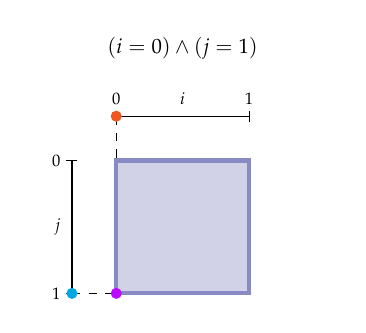
\begin{tikzpicture}[scale=1,black,x=1pt,y=1pt,every node/.style={scale=0.6}]
				\useasboundingbox (-32, -4) rectangle (80, 96);
				% Points
				\coordinate (TL) at (0, 48);
				\coordinate (TR) at (48, 48);
				\coordinate (BR) at (48, 0);
				\coordinate (BL) at (0, 0);
		
				\coordinate (ZI) at ($(TL) + (0, 16)$);
				\coordinate (UI) at ($(TR) + (0, 16)$);
				\coordinate (ZJ) at ($(TL) + (-16, 0)$);
				\coordinate (UJ) at ($(BL) + (-16, 0)$);
				\coordinate (ZJR) at ($(TR) + (16, 0)$);
				\coordinate (UJR) at ($(BR) + (16, 0)$);
		
				% Square background
				\draw[line width=0,fill=color_fill_default]
				(TL) --
				(TR) --
				(BR) --
				(BL) --
				cycle;
				
				% Interval
				\draw (ZI) -- (UI);
				\draw ($(ZI)+(0,-2)$) -- ($(ZI)+(0,2)$) node[above] {$0$};
				\draw ($(UI)+(0,-2)$) -- ($(UI)+(0,2)$) node[above] {$1$};
				\draw ($(ZI)!0.5!(UI) + (0,2)$) node[above] {$i$}
					node[above=16pt,style={scale=1.25}] {$(i = 0) \land (j = 1)$}
				;
				\draw (ZJ) -- (UJ);
				\draw ($(ZJ)+(2, 0)$) -- ($(ZJ)+(-2, 0)$) node[left] {$0$};
				\draw ($(UJ)+(2,0)$) -- ($(UJ)+(-2, 0)$) node[left] {$1$};
				\draw ($(ZJ)!0.5!(UJ) + (-2, 0)$) node[left] {$j$};
				
				% Dashed projections
				\draw[dashed]
					(ZI) -- (TL)
					(UJ) -- (BL)
					;
		
				% Grays
				\draw[line width=1.5pt, color_shaded_default]
					(TL) -- (TR) -- (BR) -- (BL) -- cycle
					;
		
				% Highlights
				\fill[color_electric_purple]
					(BL) circle(2pt)
					;
				\fill[color_flame]
					(ZI) circle(2pt)
					;
				\fill[color_cerulean_crayola]
					(UJ) circle(2pt);
			\end{tikzpicture}
		\end{column}
		}
	\end{columns}
\end{frame}

% Partial Element notation due to 1802.01170
\begin{frame}{Example | Partial Element}
	\centering
	
	We can define a \textbf{partial element} by pattern matching on a cofibration.

	\interrule

	\uncover<2->{
	For any $i : \mathbb{I} \vdash x, y : A$,
	}
	\uncover<3->{
	\begin{equation*}
		i : \mathbb{I}, \only<4->{\underbrace}{(i = 0) \lor (i = 1)}\only<4->{_\text{sometimes written $\partial i$}} \entails [(i = 0) \mapsto x, (i = 1) \mapsto y] : A \vphantom{[\underbrace{(i = 0) \lor (i = 1)}_\text{sometimes written $\partial i$}]}
	\end{equation*}
	}
\end{frame}

\begin{frame}{Path Types}
	\cleanalign{\centering}{
		\begin{gathered}
		x =_A y
		\end{gathered}
	}

	\vspace{\baselineskip}

	\interrule

	\begin{center}
	\uncover<2->{A path $p : x =_A y$ is a \alert{function} from $\mathbb{I}$ to $A$ \dots}

	\uncover<3->{\dots with \textbf{endpoints} $p\, \textbf{0} \equiv x$ and $p\, \textbf{1} \equiv y$.}
	\end{center}
\end{frame}

\begin{frame}{Example | Reflexivity, Symmetry}
	\centering
	\uncover<2->{Any self-respecting `equality' ought to be \alert{reflexive}, \alert{symmetric}, and \alert{transitive}.}
	\interrule
	\begin{columns}[onlytextwidth]
		\begin{column}{0.5\textwidth}
			\centering
			\begin{align*}
				\uncover<3->{\mathsf{refl} &\defcolon x = x}\\
				\uncover<4->{\mathsf{refl} &\equiv \lambda i.\ \uncover<5->{x}}
			\end{align*}
			\uncover<3->{for any $x : A$}
		\end{column}
		\begin{column}{0.5\textwidth}
			\centering
			\begin{align*}
				\uncover<3->{\mathsf{sym} &\defcolon (x = y) \to (y = x)}\\
				\uncover<6->{\mathsf{sym} &\equiv \lambda p.\ \uncover<7->{\lambda i.\ p \, (\neg i)}}
			\end{align*}
			\uncover<3->{for any $x, y : A$}
		\end{column}
	\end{columns}
	\vspace*{\medskipamount}
\end{frame}

\begin{frame}{Demonstration | Function Extensionality}
	\centering
	Cubical type theories let us \alert{prove} the principle of \textbf{function extensionality}:
	\begin{equation*}
		\mathsf{funext'} \defcolon \prod_{f : A \to B}\,\prod_{g : A \to B}\,\only<2->{\overbrace}{\Biggl(\prod_{x : A}\,f\,x = g\,x\Biggr)}\only<2->{^\text{pointwise equal}} \to {\only<3->{\underbrace}{(f = g)}\only<3->{_\text{equal!}}} \vphantom{\overbrace{\Biggl(\prod_{x : A}\,f\,x = g\,x\Biggr)}^\text{pointwise equal} \to \underbrace{(f = g)}_\text{equal!}}
	\end{equation*}
	\uncover<4->{Let's prove this in \alert{Agda}!}
\end{frame}

\begin{frame}{(Kan) Composition Structure}
	\centering
	\uncover<2->{We need our types to have a \textbf{composition structure}}.

	\uncover<3->{Lots of different variations!}

	\uncover<4->{Agda uses \textbf{homogeneous composition} and \textbf{transport}.}
\end{frame}

\begin{frame}{Cubical Subtypes}
	\centering
	Let $u : A$ be a \alert{partial element} in a \alert{restricted context} $\Gamma, \phi$.

	\uncover<2->{$A[\varphi \mapsto u]$ is the \textbf{cubical subtype} of elements $x : A$ such that $\varphi \implies x \equiv u$.}
\end{frame}

% CHM (1802.01170) pg 11 - we borrow notation from there, but use A instead of D(u) and the proper
% notation for substitution (like the one we saw in semantics)
\begin{frame}{Homogeneous Composition}
	\centering
	\begin{equation*}
	\inferrule*
	{
		\Gamma \entails \only<2>{\hlmathy{color_mbgreen}}{A \mathrel{\mathsf{type}}}
		\and
		\Gamma \entails \only<3>{\hlmathy{color_mbgreen}}{\varphi : \mathbb{F}}
		\and
		\Gamma, j : \mathbb{I}, \varphi \entails \only<4,8>{\hlmathy{color_mbgreen}}{u : A}
		\and
		\Gamma \entails \only<5,8>{\hlmathy{color_mbgreen}}{u_0 : A [\varphi \mapsto u[0/j]]}
	}
	{
		\uncover<6->{\Gamma \entails \alert{\mathsf{hcomp}}^j_A\,[\varphi \mapsto u] u_0 \defcolon A[\only<7>{\hlmathy{color_msgreen}}{\varphi \mapsto u[1 / j]}]}
	}
	\end{equation*}

	\uncover<8->{If $u$ and $u_0$ form an \textbf{open box}, then $\mathsf{hcomp}$ lets us \textbf{close} the box (by giving us $u_1$).}
\end{frame}

\begin{frame}[t]{Example | Transitivity}
	\begin{center}
		Let's prove \textbf{transitivity}.
	\end{center}
	\vskip\bigskipamount
	\begin{columns}
		\begin{column}{0.6\textwidth}
			\centering
			\uncover<2->{
			Suppose $x, y, z : A$.
			\vskip\medskipamount
			\cleanalign{\centering}{\begin{aligned}
				- \pathcom - &\defcolon (x = y) \to (y = z) \to (x = z) \phantom{\ (p i)}\\
				\vphantom{[\begin{smallmatrix*}[l]{(i = 0) \mapsto x}\\{(i = 1) \mapsto q\,j}\end{smallmatrix*}]} % To prevent line moving slightly up/down.
				\only<2>{{-} \pathcom {-} &\equiv {?}}
				\only<3>{{-} \pathcom {-} &\equiv \lambda p.\ \lambda q.\ {?}}
				\only<4-11>{{-} \pathcom {-} &\equiv \lambda p.\ \lambda q.\ \lambda i.\ {?}}
				\only<12>{{-} \pathcom {-} &\equiv \lambda p.\ \lambda q.\ \lambda i.\ \mathsf{hcomp}^j_A\,[\begin{smallmatrix*}[l]{(i = 0) \mapsto x}\\{(i = 1) \mapsto q\,j}\end{smallmatrix*}] (p\,i)}
			\end{aligned}}
			}
			\vskip\medskipamount
			\uncover<2-11>{
			\begin{boxybox}
				\begin{flushleft}
					\cleanalign{\centering}{\begin{aligned}
						\only<2>{\textsc{Goal: }& (x = y) \to (y = z) \to (x = z)}
						\only<3>{\textsc{Goal: }& x = z}
						\only<4->{\textsc{Goal: }& A}
					\end{aligned}}
				\end{flushleft}
			\end{boxybox}
			}
			\uncover<4-11>{
			\begin{boxybox}
				\begin{flushleft}
					\cleanalign{\centering}{\begin{aligned}
						\textsc{Boundary: }& (i = 0) \mapsto x\\
						&(i = 1) \mapsto z
					\end{aligned}}
				\end{flushleft}
			\end{boxybox}
			}
		\end{column}
		% Hint - use \fbox{...} to box around a column if you want to kinda-preview it's border.
		\begin{column}{0.4\textwidth}
			\centering
			\begin{tikzpicture}[scale=1,black,x=1pt,y=1pt,every node/.style={scale=0.6}]
				\useasboundingbox (-48, -48) rectangle (96, 96);
				% Points
				\coordinate (TL) at (0, 48);
				\coordinate (TR) at (48, 48);
				\coordinate (BR) at (48, 0);
				\coordinate (BL) at (0, 0);
		
				\coordinate (ZI) at ($(TL) + (0, 32)$);
				\coordinate (UI) at ($(TR) + (0, 32)$);
				\coordinate (ZJ) at ($(TL) + (-32, 0)$);
				\coordinate (UJ) at ($(BL) + (-32, 0)$);
				\coordinate (ZIR) at ($(BL) + (0, -32)$);
				\coordinate (UIR) at ($(BR) + (0, -32)$);
				\coordinate (ZJR) at ($(TR) + (32, 0)$);
				\coordinate (UJR) at ($(BR) + (32, 0)$);
		
				
				% Interval
				\only<4->{
				\draw (ZI) -- (UI);
				\draw ($(ZI)+(0,-2)$) -- ($(ZI)+(0,2)$) node[above] {$0$};
				\draw ($(UI)+(0,-2)$) -- ($(UI)+(0,2)$) node[above] {$1$};
				\draw ($(ZI)!0.5!(UI) + (0,2)$) node[above] {$i$}
				;
				}

				\only<5->{
				\draw (ZJ) -- (UJ);
				\draw ($(ZJ)+(2, 0)$) -- ($(ZJ)+(-2, 0)$) node[left] {$0$};
				\draw ($(UJ)+(2,0)$) -- ($(UJ)+(-2, 0)$) node[left] {$1$};
				\draw ($(ZJ)!0.5!(UJ) + (-2, 0)$) node[left] {$j$};
				}
				
				\only<7->{
					% Dashed projections
					\draw[dashed]
					(ZI) -- (TL)
					(UI) -- (TR)
					;
				}
				\only<10->{
					\draw[dashed] (ZJ) -- (TL);
				}
				\only<11->{
					\draw[dashed] (UJ) -- (BL);
				}

				\only<6->{
				% Square background
				\draw[line width=0,fill=color_fill_default]
				(TL) --
				(TR) --
				(BR) --
				(BL) --
				cycle;
				% Grays
				\draw[line width=1.5pt, color_shaded_default]
					(TL) -- (TR) -- (BR) -- (BL) -- cycle
					;
				}
				
				\only<7->{
					\fill[color_flame]
						(ZI) circle(2pt)
						(UI) circle(2pt)
						;
				}

				\only<8->{
					\draw ($(TL)!0.5!(BL)$) node[left=4pt] {$x$};
					\draw[line width=1.5pt, magenta]
						(TL) -- (BL);
					\fill[magenta]
						(TL) circle(2pt) node[above left] {$x$}
						(BL) circle(2pt) node[below left] {$x$}
						;
				}
				
				\only<9->{
					\draw ($(TR)!0.5!(BR)$) node[right=4pt] {$q\, j$};
					\draw[line width=1.5pt, magenta]
						(TR) -- (BR);
					\fill[magenta]
						(TR) circle(2pt) node[above right] {$y$}
						(BR) circle(2pt) node[below right] {$z$}
						;
				}

				\only<10->{
					\draw ($(TL)!0.5!(TR)$) node[above=4pt] {$p\,i$};
					\draw[line width=1.5pt, color_blue]
						(TL) -- (TR);
					\fill[color_electric_purple]
						(TL) circle(2pt) node[above left] {$x$}
						(TR) circle(2pt) node[above right] {$y$}
						;
					\fill[color_cerulean_crayola]
						(ZJ) circle(2pt)
						;
				}
				\only<11->{
					\draw ($(BL)!0.5!(BR)$) node[below=4pt] {$\mathsf{hcomp}$};
					\draw[line width=1.5pt, color_blue]
						(BL) -- (BR);
					\fill[color_electric_purple]
						(BL) circle(2pt) node[below left] {$x$}
						(BR) circle(2pt) node[below right] {$z$}
						;
					\fill[color_cerulean_crayola]
						(UJ) circle(2pt)
						;
				}
				% 
		
				% Highlights

				%\draw[line width=1.5pt, color_blue]
				%	(BL) -- (BR);
				%\fill[color_blue]
				%	(BR) circle(2pt)
				%	;

				%\fill[color_electric_purple] (BL) circle(2pt);
				
			\end{tikzpicture}
		\end{column}
	\end{columns}
\end{frame}

\begin{frame}{Generalized Transport}
	\centering
	\begin{equation*}
	\inferrule*
	{
		\Gamma, i : \mathbb{I} \entails \only<2>{\hlmathy{color_mbgreen}}{A \mathrel{\mathsf{type}}}
		\and
		\Gamma \entails \only<3>{\hlmathy{color_mbgreen}}{\varphi : \mathbb{F}}
		\and
		\Gamma, i : \mathbb{I}, \varphi \entails \only<4>{\hlmathy{color_mbgreen}}{A \equiv A[0/i]}
		\and
		\Gamma \entails \only<5>{\hlmathy{color_mbgreen}}{u_0 : A [0/i]}
	}
	{
		\uncover<6->{\Gamma \entails \alert{\mathsf{transp}}^i\, A\, \varphi\, u_0 \defcolon A[\only<7>{\hlmathy{color_msgreen}}{1/i}][\only<8>{\hlmathy{color_msgreen}}{\varphi \mapsto u_0}]}
	}
	\end{equation*}
\end{frame}

\begin{frame}{Example | Transport}
	\centering
	We can now \textbf{transport} a point along an \alert{equality} of types.
	\begin{align*}
		\mathsf{transport}_{A, B} &\defcolon A \equiv B \to A \to B\\
		\mathsf{transport}_{A, B} &\equiv \lambda p.\, \lambda x.\,\mathsf{transp}^i\,  (p\, i)\, \only<2>{\hlmathy{color_msgreen}}{0_\mathbb{F}}\, x
	\end{align*}
	\uncover<3->{
	Transport along a \alert{constant} path \textbf{reduces} to the input:
	\begin{align*}
		\mathsf{transportRefl} &\defcolon \only<4>{\hlmathy{color_msgreen}}{\mathsf{transport}_{A, A}\, (\mathsf{refl}\, A)\, x} = \only<5>{\hlmathy{color_msgreen}}{x}\\
		\mathsf{transportRefl} &\equiv \lambda i.\, \mathsf{transp}^i\, A\, \only<4-5>{\hlmathy{color_msgreen}}{(i = 1)}\, x
	\end{align*}
	}
\end{frame}

\begin{frame}{Higher Inductive Types}
	\centering
	Constructors of \textbf{higher inductive types} can produce points, paths, paths between paths \dots
\end{frame}

\begin{frame}{What's Not Covered Here?}
	\begin{itemize}
		\uncover<2->{\item \textbf{Glue}/\textbf{equivalence extension} types: used to prove \textbf{univalence}:}
		\begin{itemize}
			\uncover<3->{\item $(A \simeq B) \simeq (A = B)$}
			\uncover<4->{\item Nice consequences for mathematics (e.g. \alert{univalent} categories).}
		\end{itemize}
		\uncover<5->{\item \textbf{Dependent} path types: dependent functions out of the interval.}
		\begin{itemize}
			\uncover<6->{\item We can define these using $\mathsf{trans}$.}
			\uncover<7->{\item Agda defines path types \textit{in terms} of dependent path types.}
		\end{itemize}
		\uncover<8->{\item \textbf{Swan} identity types, which support \emph{judgemental} path induction.}
	\end{itemize}
\end{frame}

\begin{frame}{What's Next?}
	\begin{itemize}
		\uncover<2->{\item \textbf{Cartesian} cubical type theory: no ${\land}, {\lor}, {\neg}$, but has $(r = s)$.}
			\begin{itemize}
				\uncover<3->{\item Implemented in the experimental \textcolor{color_blue}{cooltt}.}
			\end{itemize}
			\uncover<4->{\item \textbf{Extension types}: generalized path types for user-provided cofibrations.}
			\uncover<5->{\item Other cube categories being investigated: \textbf{Dedekind}, \textbf{disjunctive}, \textbf{semicartesian}\dots}
			\uncover<6->{\item \textbf{XTT}, a non-univalent cubical type theory with \textbf{regularity} and \textbf{UIP}.}
			\uncover<7->{\item \textbf{HOTT}, a (\alert{work-in-progress}) univalent type theory with \textbf{observational} identity types.}
		\begin{itemize}
			\uncover<8->{\item $\mathsf{Id}_{A \times B}(\dots) \equiv \mathsf{Id}_A(\dots) \times \mathsf{Id}_B(\dots)$}
		\end{itemize}
	\end{itemize}
\end{frame}

\begin{frame}[plain,t]{Cubical Resources | agda/cubical}
	\centering
	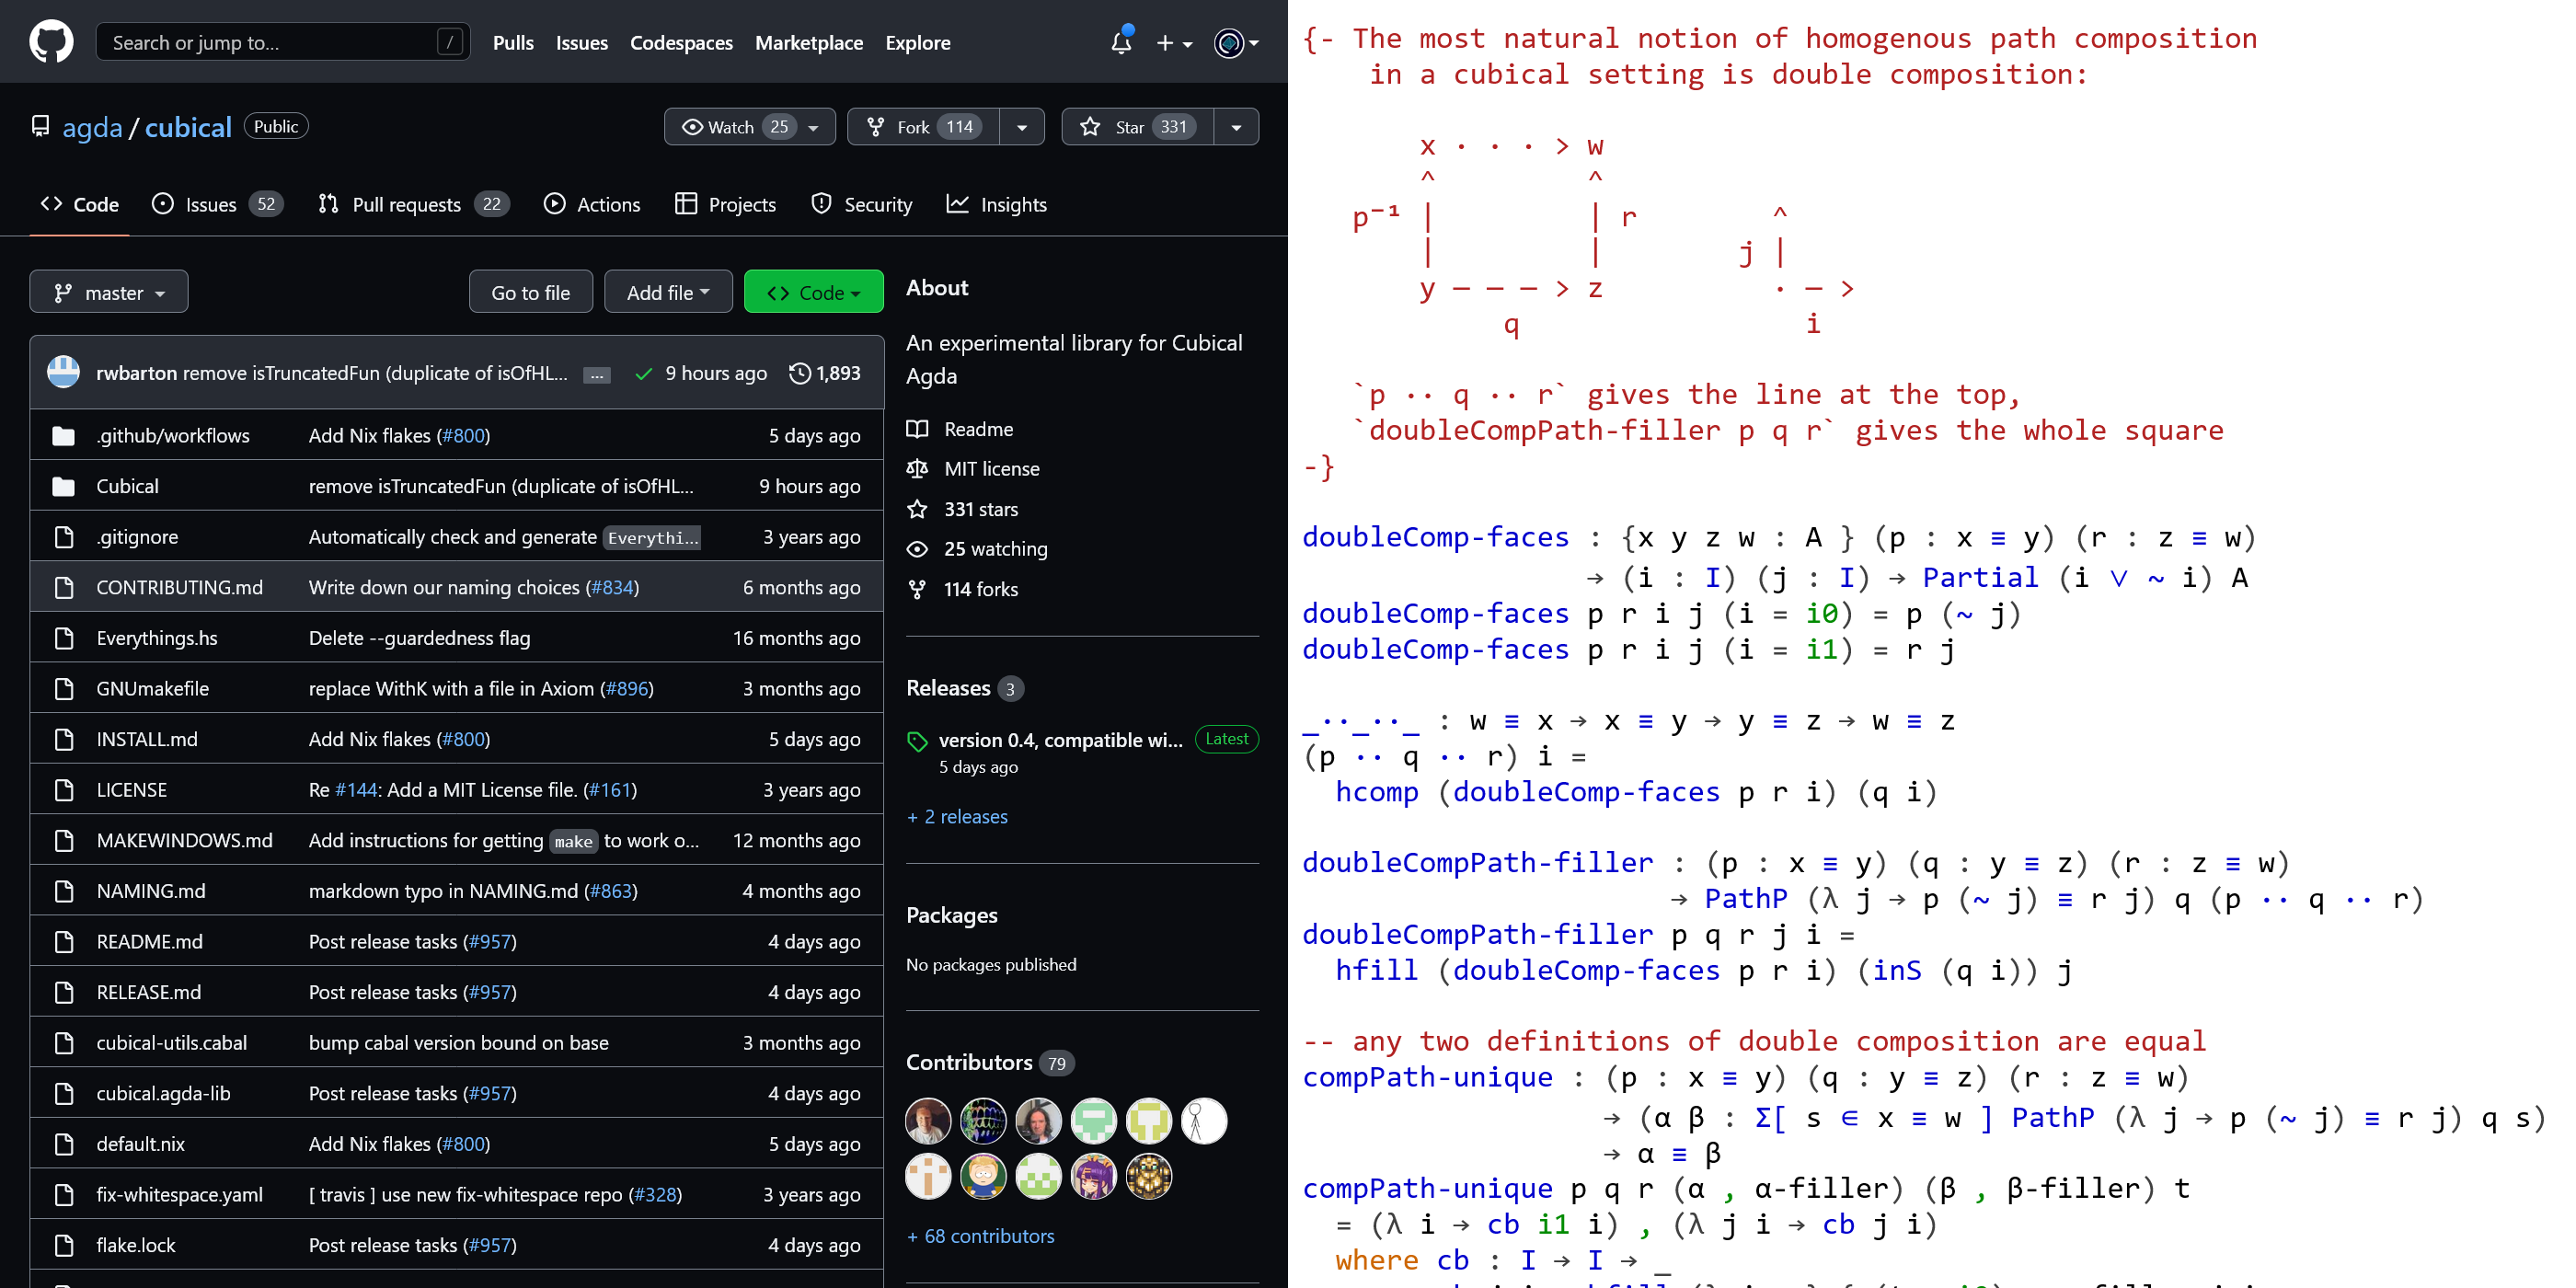
\includegraphics[width=0.9\textwidth]{../res/agda-cubical.png}

	github.com/agda/cubical

\end{frame}

\begin{frame}[plain,t]{Cubical Resources | The 1lab}
	\centering
	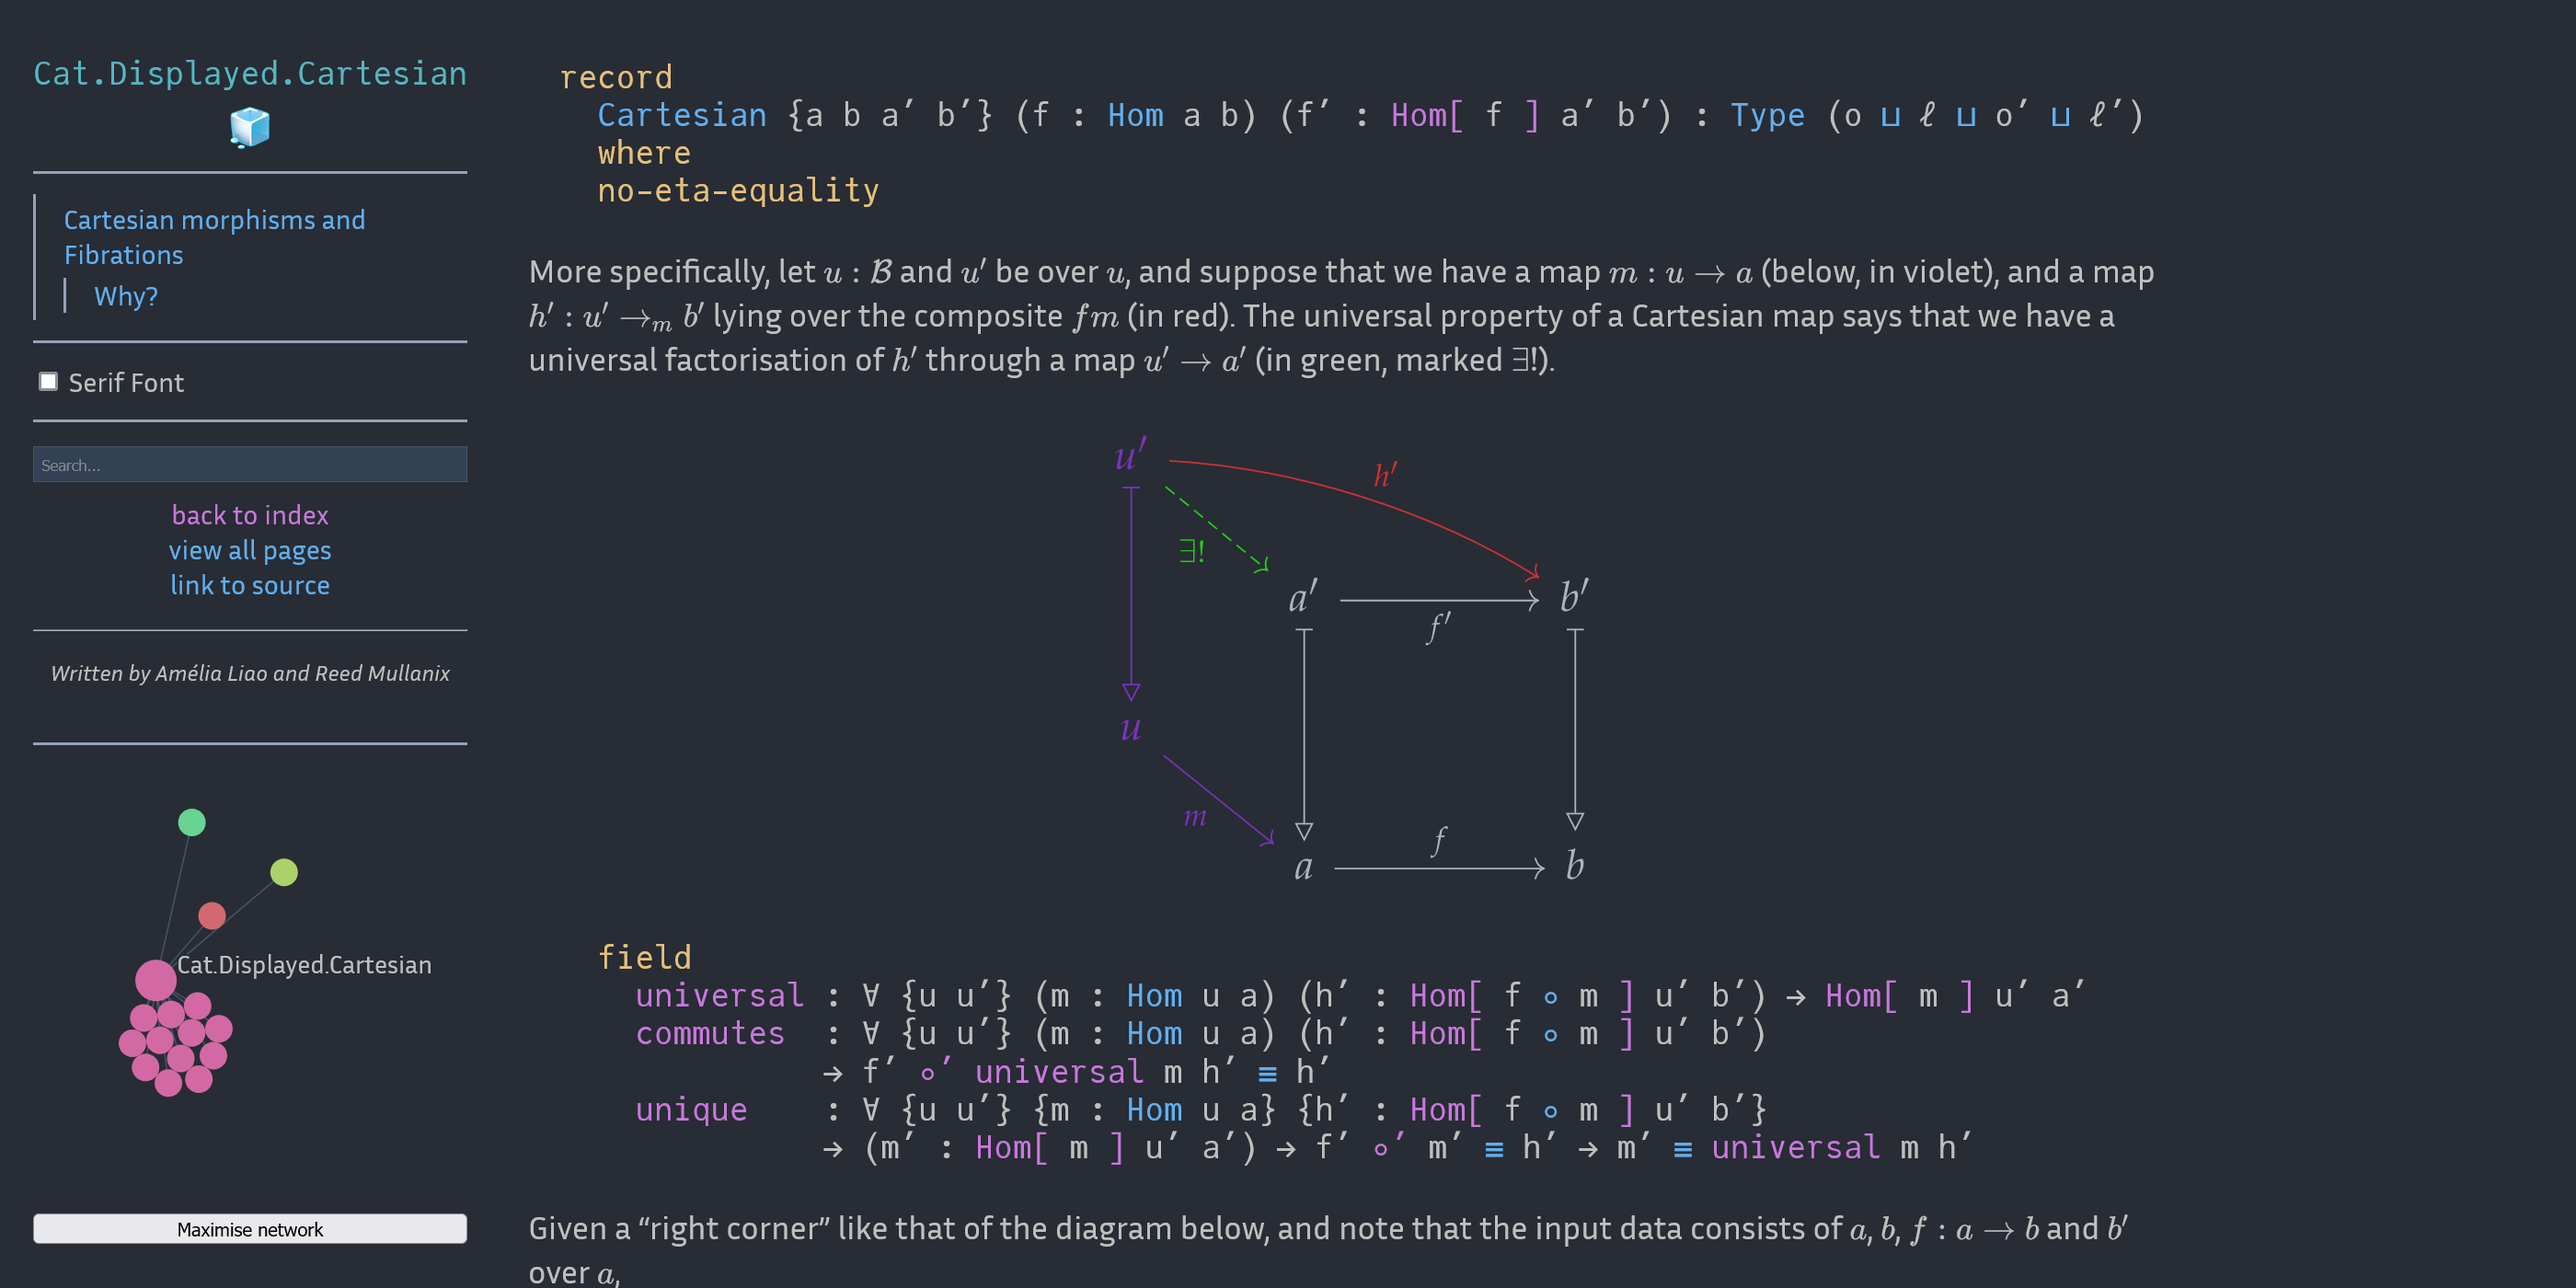
\includegraphics[width=0.9\textwidth]{../res/1lab-cartesian.png}

	1lab.dev
\end{frame}

\begin{frame}[plain]
	\centering
	Thank you!
\end{frame}
\begin{frame}[shrink=50]{Bibliography}
	\nocite{*}
	\printbibliography[heading=none]
\end{frame}
\addtocounter{framenumber}{1}
\end{document}

